\documentclass[conference]{IEEEtran}

% Write an eight page technical paper describing your project in the style of an IEEE Visualization Technical Paper (other formats may be acceptable with pre-approval).

% Sections you should plan to include are: abstract, introduction, related work (adapt your literature review for this), implementation, results, future directions, and references.

% Your paper should include figures and images as appropriate.

% A complete draft of your paper, including figures and images, must be submitted in advance of the final paper deadline.

% Your draft should be a complete paper that is as strong and polished as you can make it.

% Aim for something that you believe is ready for submission to a conference or journal.

% The course instructor will serve as reviewer for these papers and make suggestions as to how they might be improved.

% You may submit earlier, not necessarily complete, drafts of your paper if you would like feedback earlier in the writing process.

% Correct spelling and grammar count in all submitted work, so check them before you hand anything in.



\usepackage{epsfig}

% Example figure
%\begin{figure}[ht]
% \centering
% \includegraphics[scale=.8]{old.png}
% \caption{}
% \label{old}
% \end{figure}


\begin{document}

\title{SwarmVis: a Tool for Visualizing Swarm Systems}

\author{\IEEEauthorblockN{Don Miner}
\and
\IEEEauthorblockN{Niels Kasch}
}
\maketitle


\begin{abstract}
Abstract 
\end{abstract}

\section{Introduction}
Swarm systems are a collection of agents that exhibit some collective behavior. Examples of these systems include: social animals (e.g. bees, ants, schooling fish, migrating geese), particles in liquids,  and multi-robot systems. Visualizing swarm systems (swarms) effectively is difficult due to the large number of individual agents contained. A typical swarm's high density and chaotic motions amplify the complexity of swarm visualization. Effective swarm visualizations are needed to provide insight into swarm behavior and inspect local interactions.
A well defined set of visualization techniques would provide researchers with these insights.

Crude visualization techniques plot the position of each agent in space as seen with a Reynolds boid flock\cite{reynolds1987} in Figure \ref{old}. A still image only shows the location of individual agents and does not convey important information such as the direction, velocity, and previous positions.
We have implemented \textit{SwarmVis}, a toolkit for visualizing swarms, that goes beyond the simple plotting technique to solve these problems. The toolkit aims to provide visualization techniques that allow researchers to interactively investigate swarms so that researchers will be able to study interactions, fine-grained movements, and swarm behavior.

\begin{figure}[ht]
\centering
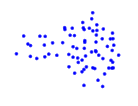
\includegraphics[scale=1]{images/basic.png}
\caption{ }
\label{old}
\end{figure}

The goal of SwarmVis is to facilitate, through visualization, the detailed analysis of emergent behavior that results from swarm systems. In order to satisfy this objective, we have created a software toolkit with the following high-level application goals and requirements in mind:
\begin{itemize}
\item The toolkit shall visualize swarms using a series of still images (i.e. a video) embedded in an interactive framework that has features such as pausing, slowing down and rewinding of frames.
\item Agent position, direction and velocity shall be conveyed through both still images and videos generated from the software.
\item The toolkit shall provide a variety of built-in visualization techniques that are useful in visualizing swarm systems.
\end{itemize}

In this paper, we discuss previous work in swarm system visualization,
some of which has provided inspirations for the techniques in SwarmVis.
Then, we discuss the implementation details of the user interface and graphical visualization.
We conclude with an overview of the projects and an analysis of its effectiveness.
A brief user guide for compiling, running and loading data in SwarmVis is provided in the appendix.

\section{Related Work}
\cite{Luke}


\section{Implementation}
Introduction to implementation here. Talk about how project is set up, what code and frameworks we used. Brief overview of the
interface. Say something about the general way visualizations are made.

\subsection{Visualizations}
Enumerate the visualizations available


\section{Results}
Results here

\section{Future Work}
SwarmVis is a complete application that has accomplished all the goals that we set out to achieve. 
However, there are a few user interface changes that would make usability better.
Also, we would like SwarmVis to visualize the instantaneous velocity of agents since this information is not explicitly present in the
graphical display. These future improvements are enumerated in this section.

In the future, we would like to make it easier to select agents and determine which agents are which in the graphical display.
To facilitate this, we hope to be able to show text labels that are adjacent to the agent in the visualization window.
These labels can show the name of the agent in the agent list.
Also, the ability to click agents in the visualization window will allow for greater interactivity and easier modification of agent-level colors and effects.

Currently, each visualization effect is controlled by a separate procedure.
Therefore, separate agent lists are kept in the Agents tab, the Tracks tab and the Types tab.
To make changes to an effect requires using that effect's tab and any changes made (e.g., color) are not reflected in the other lists.
Having an interactive global agent list that displays all necessary information will enable users to modify
the colors and effects on groups of agents more effectively. 

We also plan on adding the feature to change the representation of the agent itself to better display direction. Currently, direction is
inferred by the user by viewing the agents' tail, which may not be effective in every situation.
If agents were represented as three-dimensional arrowheads or perhaps other glyphs,
still images would convey very clearly the direction the agent is going on.

Finally, we plan on making SwarmVis extendable through a plug-in type framework. Any new visualization effects that are added
to SwarmVis must be hard coded into the source. This is not intuitive for a user that does not have knowledge of the source code
who wishes to add his own visualization to SwarmVis. Plug-ins could be simple programs that take the agent data as input and return
what the plug-in would like to have drawn on the screen. For example, the agent trails effect could be implemented as a plug-in, such
that it returns a list of lines to be drawn. A plug-in user interface will have to be implemented that allows users to manage plugins,
as well as use them. There should be some way for the plug-ins to interface with the global agent list to add informations to columns
and access information.


\bibliographystyle{IEEE}
\bibliography{cmsc636-swarmvis}

\appendix[User Guide]

\subsection{Compiling and Running}
SwarmVis was created to run on Unix-like systems, such as Mac OS X and GNU/Linux.
The following programs are required to compile SwarmVis:
\begin{itemize}
\item Qt 4.2
\item gcc/g++ 4.2.2
\item make
\end{itemize}
Note that some libraries from Qt4.2 may be needed to run SwarmVis in binary form.
We have tested SwarmVis on Mac OSX 10.5 and openSUSE Linux 11.

Run \texttt{qmake}, then run \texttt{make}, both in the root directory, to compile SwarmVis.
A binary will be created in the \texttt{bin/} directory. Execute this binary to run SwarmVis.

\subsection{Data File Format}
SwarmVis requires a specific file format for data sets that are to be loaded. The agents' position data is segmented into
separate files that each represent a single time step. These files are space-delimited data, with
each row representing an agent. For example, a swarm system with 100 agents depicted over 500 time steps
will have 500 files in a folder, each with 100 lines.

Each row entry in a file follows a format as well. The first two or three  columns (depending on dimensionality) are the
position data $(X, Y)$ or $(X, Y, Z)$, respectively. The last column is reserved for the group label, which may be used to pass
group membership data to SwarmVis.
For example, a well-formed line that conveys a three-dimensional
position with group information could be:
\begin{quote}
\texttt{10.15 5.24 84.85 CornerAgent}
\end{quote}
The listing of agents in each file should be stable. That is, the third line in one file and the third line in another file
should represent the same agent.

A plain-text information file containing important meta-data must accompany the frame files in the same directory.
The following variables must be defined (i.e., \texttt{VARNAME = VALUE}) in this file in order for the data to be loaded appropriately:
\begin{itemize}
\item \texttt{DIMENSIONS} (\texttt{2} or \texttt{3})
\item \texttt{AGENTS} (the number of agents)
\item \texttt{FRAMES} (the number frames/time steps)
\item \texttt{RANGEX} (the maximum X value)
\item \texttt{RANGEY} (the maximum Y value)
\item \texttt{RANGEZ} (the maximum Z value)
\item \texttt{AGENTTYPES} (\texttt{1} to track agent types, \texttt{0} if not)
\end{itemize}
At the bottom of this file, the keyword \texttt{FILES} must appear, followed by a list of frame files, in temporal order. The number
of files listed here must equal the number specified by the \texttt{FRAMES} variable. Also,
the number of lines in every file must match the number specified by the \texttt{AGENTS} variable. Below is a sample info file:
\begin{verbatim}
     DIMENSIONS = 3
     AGENTS = 150
     FRAMES = 446
     RANGEX = 600
     RANGEY = 600
     RANGEZ = 600
     AGENTTYPES = 1

     FILES
     frame000001.txt
     frame000002.txt
     ...
     frame000446.txt
\end{verbatim}

To load a data set in the SwarmVis application, navigate to ``Load Data" and select the info file.

\end{document}


